\chapter{Análisis} \label{analisis}
\epigraph{\textit{Research is what I'm doing when I don't know what I'm doing.   
	}}{\textit{— Wernher von Braun, NASA engineer}}
	\vspace*{8cm}
	\begin{center}
		\centering
		\includegraphics[width=10.5cm]{example-image}
    \end{center}
\thispagestyle{empty}
\newpage
\vspace*{2cm}

\section{Estudio de factibilidad}
En esta sección del trabajo terminal, abordaremos la factibilidad técnica y económica que tendrá la implementación de la solución propuesta. Para ello se dará respuesta a las siguientes preguntas sobre la factibilidad del sistema.

\textbf{\textit{¿Este sistema implementará alguna tecnología que no se haya empleado previamente?}}\newline
Para el desarrollo del sistema no requerirá alguna tecnología que no se haya implementado anteriormente, ya que los usuarios deberán contar con un dispositivo móvil para realizar las actividades necesarias para el funcionamiento de este. 

\textbf{\textit{¿El sistema puede integrarse dentro de alguna organización?}}\newline
El sistema se plantea como un sistema independiente, pero, puede hacerlo adaptando el sistema para que sea consumido por otros que estén en la organización que lo use.

\textbf{\textit{Considerando gastos, tecnología, conocimiento y tiempo ¿El desarrollo del sistema es conveniente?}}\newline
La respuesta es sí, ya que la tecnología que implementará tiene una gran comunidad y tiene años en el mercado, lo único necesario es acceso a un equipo de computo y tener acceso a internet, con lo que ya se cuenta. Los problemas son la falta de conocimiento técnico con algunos temas, sin embargo, el tiempo y apoyándose con la comunidad de desarrolladores que tiene las tecnologías a usar, se puede superar este problema, por otro lado puede que algunas tecnologías tengan algún costo, pero como se tiene acceso a una cuenta universitaria, existen descuentos o inclusive el uso gratuito de la tecnología que se requiera.

Por lo tanto, podemos concluir que el sistema es factible de manera técnica y económicamente.
\subsection{Herramientas necesarias para el desarrollo del sistema}

\begin{longtable}{|m{1.7cm}|c|c|c|c|}
\hline
\rowcolor[HTML]{3531FF} 
\multicolumn{1}{|c|}{\cellcolor[HTML]{3531FF}{\color[HTML]{FFFFFF}\centering Nombre}} & \multicolumn{1}{c|}{\cellcolor[HTML]{3531FF}{\color[HTML]{FFFFFF} Multiplataforma}} & \multicolumn{1}{m{2cm}|}{\cellcolor[HTML]{3531FF}{\color[HTML]{FFFFFF} Buena presentación}} & \multicolumn{1}{m{4cm}|}{\cellcolor[HTML]{3531FF}{\color[HTML]{FFFFFF} Soporte para cualquier proceso UML y base de datos}} & \multicolumn{1}{m{3cm}|}{\cellcolor[HTML]{3531FF}{\color[HTML]{FFFFFF} Familiarización con la herramienta}} \\ \hline
\endfirsthead
\hline
\rowcolor[HTML]{3531FF}\multicolumn{1}{|c|}{\cellcolor[HTML]{3531FF}{\color[HTML]{FFFFFF}\centering Nombre}} & \multicolumn{1}{c|}{\cellcolor[HTML]{3531FF}{\color[HTML]{FFFFFF} Multiplataforma}} & \multicolumn{1}{m{2cm}|}{\cellcolor[HTML]{3531FF}{\color[HTML]{FFFFFF} Buena presentación}} & \multicolumn{1}{m{4cm}|}{\cellcolor[HTML]{3531FF}{\color[HTML]{FFFFFF} Soporte para cualquier proceso UML y base de datos}} & \multicolumn{1}{p{3cm}|}{\cellcolor[HTML]{3531FF}{\color[HTML]{FFFFFF} Familiarización con la herramienta}} \\ \hline
\endhead
\multicolumn{5}{c}{Sigue en la página siguiente.}
\endfoot
% aquí añadimos el fondo de la última hoja.
\endlastfoot

Umbrello 2.32 & Si & Si & No & No \\ \hline
Rational Rose & Si & Si & Si & No \\ \hline
Visual Paradigm & Si & Si & Si & Si \\ \hline

\caption{Herramientas CASE}
\label{table:Case}
\end{longtable}
Con la tabla \ref{table:Case} se da por hecho que se usará el Software de Visual Paradigm ya que cumple las características requeridas para realizar los diseños correspondientes del sistema.

\subsection{Elección de software}

\begin{table}[!htb]
\begin{tabular}{|c|c|c|c|}
\hline
\rowcolor[HTML]{3531FF} 
{\color[HTML]{FFFFFF} Nombre} & {\color[HTML]{FFFFFF} Orientado a objetos} & {\color[HTML]{FFFFFF} Multiplataforma} & {\color[HTML]{FFFFFF} Famialiarización con el lenguaje} \\ \hline
Dart & Si & Si & Si \\ \hline
Python & Si & Si & Si \\ \hline
Java & Si & Si & No \\ \hline
\end{tabular}
\caption{Lenguajes de programación}
\label{table:Programacion}
\end{table}
Los lenguajes a utilizar para desarrollar el sistema son dos: Dart y Python. Java no se usará porque no se está familiarizado con el lenguaje y por otro lado, consume recursos ya que esté utiliza una máquina virtual para poder ejecutar las aplicaciones a desarrollar y que en equipos poco potentes la experiencia de usuario pueda verse afectada. Sin embargo, Dart y Python son opciones viables ya que cada uno tiene frameworks que facilitarán la creación del sistema, a continuación se presentarán características de los lenguajes de programación electos.

\subsubsection{Dart y Flutter}
Dart es un lenguaje de programación orientado a objetos y definido por clases. La maquina virtual de Dart cuenta con un motor de ejecución \acrfull{JIT}. Al escribir y depurar una aplicación, la compilación \acrshort{JIT} permite la "recarga en caliente" con la que se inyectar modificaciones a los archivos de origen en una aplicación en ejecución \cite{Vega2019}. 

\begin{figure}[!htb]
    \centering
    
\includegraphics[scale=0.1]{TT/img/analisis/dartlogo.png}
    \caption{Logo de Dart}
    \label{graphic:DartLogo}    
\end{figure}

El motor de ejecución de Dart puede ser \acrfull{AOT} compilado en código nativo rápido y predecible, lo que permite que casi todo Flutter sea escrito en Dart. Esto no sólo hace que Flutter sea rápido, sino que prácticamente todo (incluidos todos los widgets) se puede personalizar. Dart facilita la creación de animaciones y transiciones suaves que se ejecutan a 60fps.

Además, Dart es declarativo y, por lo tanto, permite evitar la necesidad de un lenguaje de diseño declarativo separado como \Gls{JSX} o \Gls{XML}, o constructores de interfaz visual separados. Todo el diseño se realiza en un idioma y en el mismo archivo, por lo que es fácil tener herramientas avanzadas que hacen que el diseño y la construcción del diseño sean muy rápidos.
\newline

\textbf{Todo es un Widget}

El 4 de diciembre de 2018, Google anunció la primera versión estable del framework Flutter. Flutter permite un desarrollo rápido para plataformas móviles y últimamente para plataformas web y de escritorio. 
\begin{figure}[!htb]
    \centering
    
\includegraphics[scale=0.3]{TT/img/analisis/flutterlogo.png}
    \caption{Logo de Flutter}
    \label{graphic:FlutterLogo}    
\end{figure}
El bloque fundamental de flutter es el Widget: todo es un widget. El desarrollo de Flutter consiste en describir el diseño de la aplicación en el dispositivo, componiendo, ensamblando y creando widgets a partir de otros. Todos estos están organizados en un árbol, que tiene como raíz el método buid() del Widget de la aplicación principal.

Cada hoja del árbol es hija de su widget padre, que se construye después de sus hijos. Una página de documentación dice: "Un widget es una descripción inmutable de parte de una interfaz de usuario" \cite{Flutter2020}.

Sin embargo, hay muchos tipos de widgets en Flutter y durante el desarrollo común no se puede ver ni tocar todos. Una cadena de texto es un widget(\textbf{Text}), pero también lo es su estilo (\textbf{TextStyle}), que define cosas como tamaño, color, fuente y tamaño. 

\begin{figure}[!htb]
    \centering
    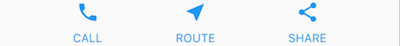
\includegraphics[scale=1]{TT/img/analisis/UIElementA.png}
    \caption{Interfaz gráfica.}
    \label{graphic:UIPart}
\end{figure}
\begin{figure}[!htb]
    \centering
    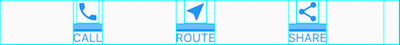
\includegraphics[scale=1]{TT/img/analisis/UIElementB.png}
    \caption{Identificación de los elementos de la interfaz gráfica.}
    \label{graphic:UIElements}
\end{figure}
\begin{figure}[!htb]
    \centering
    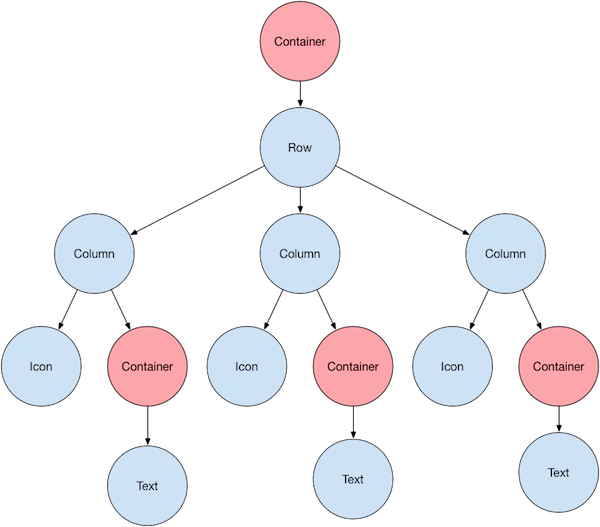
\includegraphics[scale=0.6]{TT/img/analisis/UIElementC.png}
    \caption{Estructura de árbol de un conjunto de Widgets.}
    \label{graphic:UITree}
\end{figure}
Hay Widgets que representan cosas, otros que representan características (como TextStyle) e incluso otros que realizan acciones. Se pueden crear widgets complejos combinando muchos más simples, y una aplicación es en realidad el widget más grande de todos (generalmente llamado MyApp) que contiene todos los demás widgets. 

En la figura \ref{graphic:UITree} se muestra el árbol de widgets que subyace al elemento UI mostrado. La interfaz de usuario es una fila simple que contiene 3 botones con un icono y una descripción de cada uno. Esto se traduce en la estructura del widget al tener una repetición de 3 estructuras idénticas, construyendo el botón en si, todo configurado en una fila contenida en un widget contenedor que permite establecer algunas propiedades de dimensión.

Para ver un ejemplo en código, ir hacia el apéndice \ref{aped.A}

\subsubsection{Python y FastApi}

\section{Metodología}
Para este trabajo terminal se utilizará la metodología de desarrollo rápido de aplicaciones (DRA), dado que el tiempo de desarrollo es corto, esta metodología permite centrarse en el producto final, hace hincapié en el desarrollo de prioridades y la definición de los plazos de entrega, si estos empiezan a atrasarse permite la reducción de requisitos para el ajuste y de esta manera no aumentar la fecha limite de entrega. Por otro lado la participación de los usuarios es necesaria para el diseño del sistema.\cite{dra}

\begin{figure}[!ht]
    \centering
    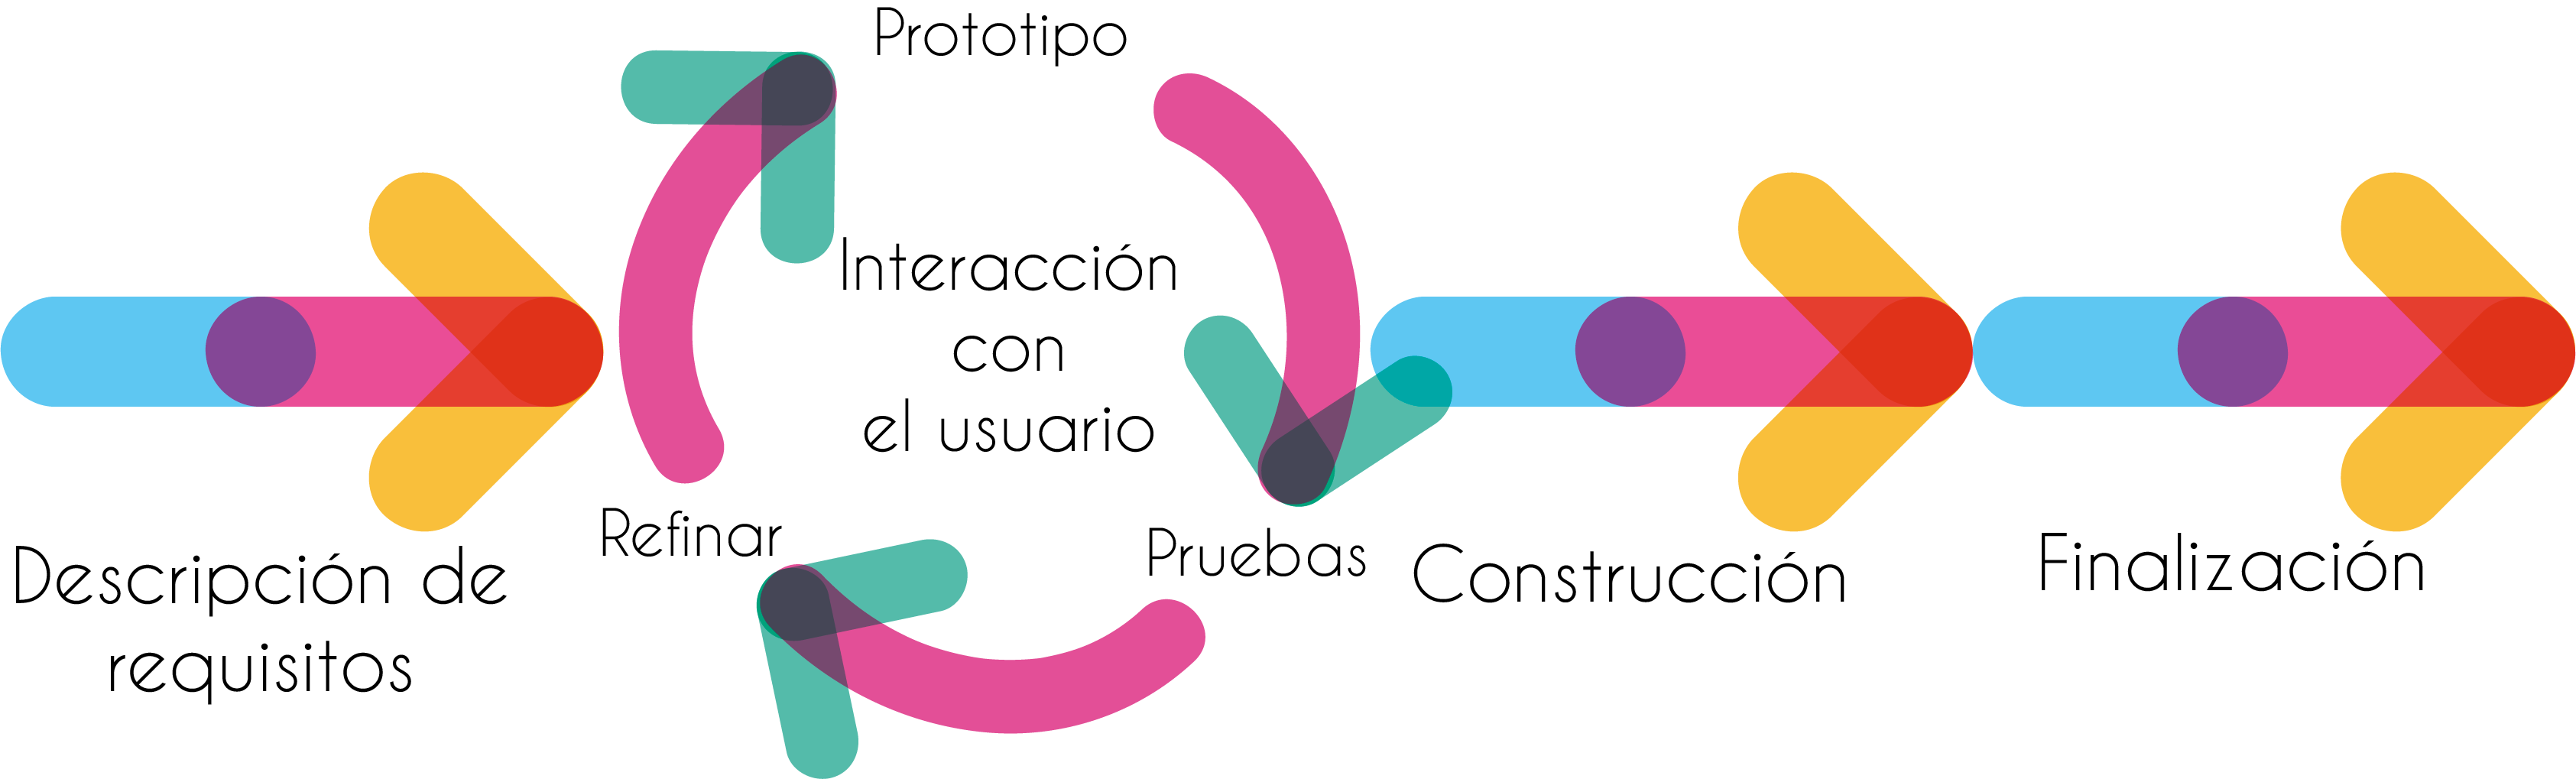
\includegraphics[scale=0.50]{TT/img/metodología/RAD.png}
    \caption{Desarrollo rápido de aplicaciones}
    \label{graphic:RAD}
\end{figure}
\section{Requerimientos}

\subsection{Requerimientos funcionales}

\subsection{Requerimientos no funcionales}

